\documentclass{beamer}
\graphicspath{{../graphics/}}
\usepackage{listings}
\usepackage{ulem}
\usepackage{subcaption}
\captionsetup{compatibility=false}
\usepackage[linesnumbered]{algorithm2e}
\usepackage{multicol}

\newcommand{\linespace}{\vspace{1em}}

\mode<presentation>
{
  \usetheme{Darmstadt}
  \setbeamertemplate{footline}[frame number]
  \setbeamertemplate{navigation symbols}{}
  \setbeamercovered{transparent}
}

\AtBeginSection[]
{
   \begin{frame}
        \frametitle{Indhold}
        \tableofcontents[sectionstyle=show/hide,subsectionstyle=show/show/hide]
   \end{frame}
}

%\usepackage[danish]{babel}
\usepackage[T1]{fontenc}

\usepackage[utf8]{inputenc}

\usepackage{times}

\usepackage{tikz}
\usepackage{3dplot}
\usepackage{multirow}

\title[Mapping med Lego-robot]{Mapping med Lego-robot}

\subtitle{SW505E13}

\author[SW505E13]{Mikkel Sand\o ~Larsen, \and Bruno Thalmann, \and Stefan Marstrand Getreuer Micheelsen, \and Stefan Thilemann, \and Mikael Elki\ae r Christensen, \and Anders R. Nielsen}

\institute[Aalborg University]
{
  Department of Computer Science\\
  Aalborg University}

\date[CFP 2003]{31. Januar 2014}

\begin{document}

%--------------------------------------------------
%     INTRODUKTION
%--------------------------------------------------

\begin{frame}
  \titlepage
\end{frame}

\begin{frame}
    \frametitle{Indhold}
    \tableofcontents[sectionstyle=show/show,subsectionstyle=hide/hide/hide]
\end{frame}

\section{Overblik}

\subsection{Multi-project}
\begin{frame}{Overview of the multi-project}
	\begin{itemize}
		\item Management of the multi-project
		\item Structure of the multi-project
	\end{itemize}
\end{frame}

\begin{frame}{Management of the multi-project}
	The multi-project consists of
	\begin{description}
		\item[Students:]{60}
		\item[Groups:]{16}
	\end{description}

	Development method: Scrum
	\begin{description}
		\item[Sprints]{Project split into four sprints}
		\begin{itemize}
			\item[Sprint 1] 24-02-2014 -- 19-03-2104 
			\item[Sprint 2] 20-03-2014 -- 14-04-2104
			\item[Sprint 3] 15-04-2014 -- 07-05-2104
			\item[Sprint 4] 08-05-2014 -- 27-05-2104
		\end{itemize}
	\end{description}
\end{frame}

\begin{frame}{Roles and responsibilities}
	Roles assigned on multi-project level and their responsibilities
	\begin{description}
		\item[Scrum Master] Chairing Scrum meetings and coordination of groups and meetings.
		\item[Sprint End Specialist] Coordinator and chairman of sprint review meetings.
		\item[Client Contact] Responsible for all communication to and from the clients.
	\end{description}
\end{frame}

\subsection{Structure}
\begin{frame}{Structure of the multi-project}
\includegraphics<1>[height=.9\textheight]{pres/scrumofscrums}
\end{frame}

\section{Løsningsmetoder}
%Løsningsmetoder
\subsection{Platform}
\begin{frame}
\frametitle{Lego Mindstorms}
\begin{itemize}
\item Tilgængelighed
\item Nemt at gå til
\item Stort udvalg af sensorer
\item Mange muligheder ift. styring
\end{itemize}
\end{frame}

\begin{frame}
\frametitle{API}
\begin{itemize}
\item NXC
\begin{itemize}
\item NXC er et C-lignende sprog med gode indbyggede funktioner
\item NXC har gode indbyggede funktioner til fejlfinding
\end{itemize}
\item MindSqualls
\begin{itemize}
\item Et .NET bibliotek skrevet i C\#
\item Tillader nem direkte kommunikation med sensorer og motorer
\end{itemize}
\end{itemize}
\end{frame}
\subsection{Sensorer og Motor}
\frametitle{Valgt sensor og motor}
\begin{frame}
\frametitle{Valgt afstandssensor}
\center
\includegraphics[width=110px, clip=true, trim = 0px 90px 0px 0px]{sensor/us}
\includegraphics[width=110px]{sensor/infrared_sensor}
\begin{itemize}
\item Begge har en afvigelse på $\pm$ 3 cm
\item Den ultrasoniske sensor har en range på 20-170 cm
\item Den infrarøde sensor har en range på 10-56 cm
\end{itemize}
\end{frame}
\begin{frame}
\frametitle{Valgt motor}
\center
\includegraphics[width=110px]{sensor/lego_motor}
\begin{itemize}
\item Testet med Motor Control
\item Store afvigelser i testen på op til +7 og -4 grader
\item Lokaliseringen skal afhjælpe upræcisionen
\end{itemize}
\end{frame}
\subsection{Lokalisering}
\begin{frame}
\frametitle{Valg af Kinect}
\begin{itemize}
\item Nem tilslutning til PC
\item RGB-kamera og Dybdesensor
\item Gode udviklingsværktøjer
\item Tilgængelig gennem universitetet
\item Colortracking
\end{itemize}
\end{frame}
\subsection{Mapping}
\begin{frame}
\frametitle{Occupancy grid}
\begin{itemize}
\item Til at kortlægge har vi valgt at bruge \textit{occupancy grid} algoritmen
\item \textit{Occupancy grid} er en familie af algoritmer som gør det muligt at generere konsistente kort
\item \textit{Occupancy grid} opdeler kortet i celler og tildeler en binær stokastisk variabel til hver celle
\end{itemize}
\end{frame}
%Robottens design
\section{Robottens design}
\subsection{Præsentation af designet}
\begin{frame}
\frametitle{Overordnet}
\begin{center}
\includegraphics[scale=0.15]{whalle}
\end{center}
\end{frame}

\begin{frame}
\frametitle{Gearing}
\begin{center}
\includegraphics[scale=0.13]{whalle_with_gearing_expl2}
\end{center}

\end{frame}

\subsection{Overvejelser}
\begin{frame}
\frametitle{Gearing}
\begin{itemize}
\item Gearing på hjul blev fjernet
\item Mere simpelt design
\item Unødvendigt med tårn til sensorer
\item En simplere løsning:
\begin{itemize}
\item Montere sensoren direkte på robottens krop
\item Rotere robotten når der skal måles
\end{itemize} 
\item Mindre kompleks robot design er formentlig lettere at arbejde med
\end{itemize}
\end{frame}



\section{Teori}
\subsection{Grundlæggende}
\begin{frame}{Occupancy Grid}
\begin{figure}[h] % Kørselsmiljø og et occupancy grid
\centering
	\begin{subfigure}[b]{.48\textwidth}
	\centering
	\includegraphics[width=\textwidth]{verden/oppefra_m_walle}
	\caption{Aktuelt Kørselsmiljø.}
	\label{map:world}
	\end{subfigure}
	\hfill
	\begin{subfigure}[b]{.48\textwidth}
	\centering
	\includegraphics[width=\textwidth]{verden/occupancy_grid_verden}
	\caption{Occupancy Grid.}
	\label{map:occupancy_grid}
	\end{subfigure}

\end{figure}
\end{frame}
\begin{frame}{Bayes Regel}
Opdatering af troen på en proposition ved ny evidens
\[
\begin{split}
P(h \mid e) = \frac{P(e \mid h) \times P(h)}{P(e)}
\end{split}
\]
\end{frame}

\begin{frame}{Log Odds}
\begin{figure}
\centering \includegraphics[scale=.2]{LogOdds}
\label{logoddsimg}
\end{figure}

%Log odds er en metode der kan benyttes for at undgå, at komponenterne i Bayes Regel enten bliver definitivt sande eller falske.
%
%Der kan derfor indføres en funktion, \textit{log odds ratio}, som mapper sandsynlighedsværdierne fra $[0;1]$ til $[-\infty;\infty]$.
%Oddset for tilstand $x$ er defineret som forholdet mellem sandsynlighederne for $x$ og $\lnot x$: 

\begin{tabular}{ p{0.5\linewidth} p{0.5\linewidth} }
$ l(x) = \log \frac{p(x)}{1 - p(x)} $ & 
$ bel_t(x) = 1 - \frac{1}{1 + exp\{l_x\}}\label{logodds:bel} $
\end{tabular}
\end{frame}

\subsection{Occupancy Grid}

\begin{frame}{Binært Bayes Filter}
Kan bruges når verdenens tilstand er statisk

\begin{algorithm}[H]
\textbf{BinaryBayesFilter($l_{t-1}, z_t$)} \\
\Indp $l_t = l_{t-1} + \log \frac{p(x \mid z_t)}{1-p(x \mid z_t)} - \log \frac{p(x)}{1-p(x)}$ \\
\Return{$l_t$}
\end{algorithm}
\end{frame}

\begin{frame}{Occupancy grid}
\begin{algorithm}[H]
OccupancyGridMapping(\{$l_{t-1,i}$\}, $x_t$, $z_t$):

\ForAll{cells $ m_i $}
{
\eIf{$ m_i $ is in the perceptual field of $ x_t $}
%then
{ $ l_{t,i} = l_{t-1,i} $ + \textbf{inverse\_sensor\_model} $( m_i, x_t, z_t ) - l_0$\\ }
%else
{ $ l_{t,i} = l_{t-1,i}  $\\ }
}
\Return {$ \{l_{t,i}\} $}
\end{algorithm}
\end{frame}

\begin{frame}{Occupancy grid}
\begin{algorithm}[H]
OccupancyGridMapping(\{$l_{t-1,i}$\}, $x_t$, $z_t$):

\ForAll{cells $ m_i $}
{
\eIf{$ x_i = x_r$ or $y_i = y_r$}
%then
{ $ l_{t,i} = l_{t-1,i} $ + \textbf{inverse\_sensor\_model} $( m_i, x_t, z_t ) - l_0$\\ }
%else
{ $ l_{t,i} = l_{t-1,i}  $\\ }
}
\Return {$ \{l_{t,i}\} $}
\end{algorithm}
\end{frame}

\subsection{Sensormodeller}
\begin{frame}{Simpel sensormodel}

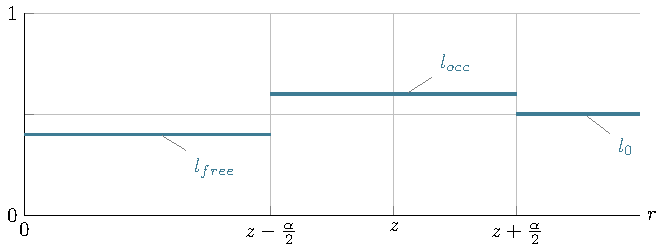
\includegraphics{simple_sensormodel.pdf}
\end{frame}

\begin{frame}{Gaussisk sensormodel}

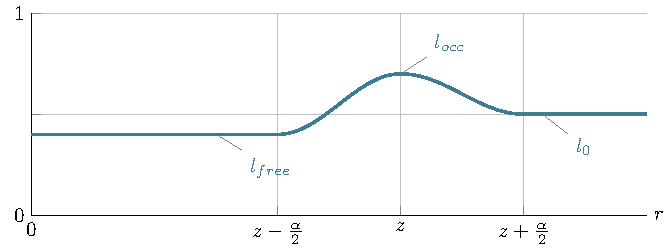
\includegraphics{gaussian_sensormodel.pdf}
\end{frame}

\begin{frame}{Sammenligning af sensormodeller}
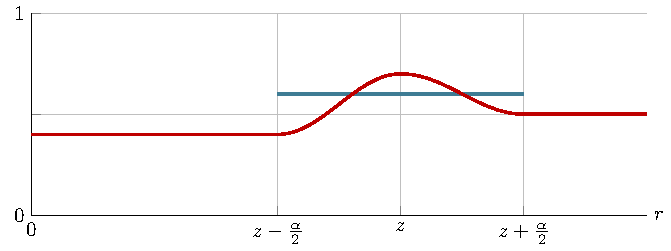
\includegraphics{combined_sensormodel}
\end{frame}


\subsection{Lokalisering}

\begin{frame}{Afstande mellem farver}

\centering
\tdplotsetmaincoords{60}{110}
\begin{tikzpicture}[scale=4,tdplot_main_coords]

%set up some coordinates 
%-----------------------
\coordinate (O) at (0,0,0);
\tdplotsetcoord{P1}{1.1}{60}{30}
\tdplotsetcoord{P2}{1.5}{40}{60}

%draw figure contents
%--------------------

%draw the main coordinate system axes
\draw[ultra thick,red,->] (0,0,0) -- (1,0,0) node[anchor=north east]{$r$};
\draw[ultra thick,green,->] (0,0,0) -- (0,1,0) node[anchor=north west]{$g$};
\draw[ultra thick,blue,->] (0,0,0) -- (0,0,1) node[anchor=south]{$b$};

\draw[-stealth,color=gray] (O) -- (P1);
\draw[-stealth,color=gray] (O) -- (P2);
\draw[-stealth,thick] (P1) -- (P2);

\draw (P1) node[anchor=west]{$C_1$};
\draw (P2) node[anchor=west]{$C_2$};

%draw projection on xy plane, and a connecting line
\draw[dashed, color=gray] (O) -- (P1xy);
\draw[dashed, color=gray] (P1) -- (P1xy);

\draw[dashed, color=gray] (O) -- (P2xy);
\draw[dashed, color=gray] (P2) -- (P2xy);

%\draw[dashed] (P1xy) -- (P2xy);
%\draw[dashed] (P2) -- (P2xy);


\end{tikzpicture}

\end{frame}

\begin{frame}{Maksimal afstand}

$$dist_{C_aC_b} = \vert C_a - C_b \vert$$

$$w_{C_aC_b} = \begin{cases}
	0 &\text{hvis } dist_{C_aC_b} > \rho \\
	1 - \frac{dist_{C_aC_b}}{\rho} &\text{hvis } dist_{C_aC_b} \leq \rho
\end{cases}$$

\end{frame}

\begin{frame}

\begin{figure}
\centering
\includegraphics[scale=.6]{tracking/emptyGrid}
\includegraphics[scale=.6]{tracking/emptyGrid_TRACK2} \\
\includegraphics[scale=.6]{tracking/emptyGrid_TRACK}

\end{figure}
\end{frame}

\begin{frame}{Problemer med metoden}
\begin{itemize}
\item Støj
\item Farveændring (lys/skygge)
\item Opdateringshastighed
\end{itemize}

\end{frame}



\begin{frame}{Filtrering af støj}
3x3 støj filter \\


$$w'_{x,y} = \begin{cases}
	0 &\text{hvis } \vert V_{x,y} \vert < \sigma \\
	w_{x,y} &\text{hvis } \vert V_{x,y} \vert \geq \sigma
\end{cases}$$ \\
hvor $$V_{x,y} = \{w \in N_{x,y} \vert w > 0 \}$$
\end{frame}

\begin{frame}{Farveændring (lys/skygge)}
Løbende opdatering af sporingsfarve.
\begin{figure}
\centering
\includegraphics[scale=.7]{tracking/emptyGrid_FILTER}
\end{figure}

\end{frame}

\begin{frame}{Opdateringshastighed}

\begin{itemize}
\item Reducere problemets størrelse
\item Robotten bevæger sig kun korte afstande mellem opdateringer
\end{itemize}

\begin{figure}
\centering

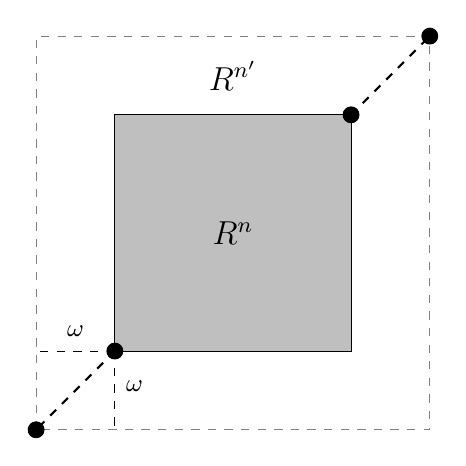
\begin{tikzpicture}[scale=.5]

%set up some coordinates 
%-----------------------
\coordinate (C1) at (0,0); % Outer top left
\coordinate (C2) at (10,10); % Outer bottom right
\coordinate (C3) at (2,2); % Inner top left
\coordinate (C4) at (8,8); % Inner bottom right

%draw figure contents
%--------------------

\draw [fill=lightgray] (C3) rectangle (C4); % Inner rectangle
\draw[dashed, color=gray] (C1) rectangle (C2); % Outer rectangle

\draw [fill] (C1) circle [radius=0.2]; % Outer top right
\draw [fill] (C2) circle [radius=0.2]; % Outer bottom left
\draw [fill] (C3) circle [radius=0.2]; % Inner top right
\draw [fill] (C4) circle [radius=0.2]; % Inner bottom left

\draw[thick,dashed] (C3) -- (C1); % Inner top right to outer top right
\draw[thick,dashed] (C4) -- (C2); % Inner bottom left to outer bottom left

\draw[dashed] (C3) -- (0,2);
\draw[dashed] (C3) -- (2,0);

\draw (5,5) node {\large $R^n$};
\draw (5,9) node {\large $R^{n'}$};

\draw (1,2.5) node {\small $\omega$}; % x1-w
\draw (2.5,1.1) node {\small $\omega$}; % y1-w

\end{tikzpicture}
\end{figure}

\end{frame}




\begin{frame}{Omregning fra punkt i billede til reelt punkt}

\centering
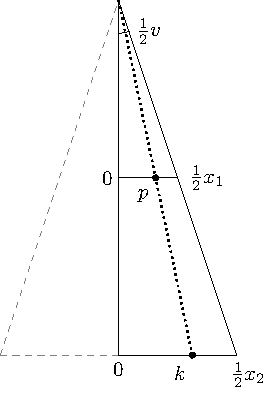
\includegraphics[scale=1]{conversion_figure}

\end{frame}









\subsection{Ruteplanlægning}

\begin{frame}{Ruteplanlægning}
Begreber:
\begin{itemize}
\item Destinationscelle
$$D = \{d \in C \vert dest(d) \}$$
\item Synlig celle
$$p(d) = \{e \in C \vert visible(d,e) \}$$
\item Cellens information gain
$$v(d) = \sum_{c \in p(d)}{0.5- \vert 0.5 - P(c) \vert}$$
\end{itemize}

\end{frame}


\begin{frame}

\begin{itemize}
\item Mængde af information gain værdier
$$V = \{v(d) \vert d \in D \}$$
\item Celler med maksimal information gain
$$Q = \{ d \in D \vert v(d) \in maxV \}$$
\item Mængde af distance mellem celler i Q
$$A = \{dist(x,q) \vert q \in Q \}$$
\end{itemize}

\end{frame}

\begin{frame}

\centering
Video demonstration

\end{frame}


\section{Design}
\subsection{Systemets Opbygning}

\begin{frame}{Hardware Komponenter}
\begin{columns}
\begin{column}{.48\textwidth}
\begin{description}
\item[Kinect]{Billed-feed til lokalisering}
\item[Robot]{Navigation i og observation af verden}
\item[PC]{Beregning af:}
\begin{itemize}
\item{kort}
\item{robot lokation}
\item{rute}
\end{itemize}
\end{description}
\end{column}
\begin{column}{.48\textwidth}
\includegraphics[width=\textwidth]{enheder}
\end{column}
\end{columns}
\end{frame}

\subsection{NXT (Robot)}

\begin{frame}{NXT Software}
Vigtigste filer og deres funktionalitet:
\begin{description}
\item[MainTask.nxc]{Main task/loop og kommunikation fra PC}
\item[Communication.nxc]{Kommunikation til PC}
\item[Navigation.nxc]{Navigation i verden}
\item[Sensor.nxc]{Observation af verden}
\item[MCTasks.nxc]{Motor Control; til bedre styring af motorer}
\end{description}
\end{frame}

\subsection{PC}

\begin{frame}{PC Software}
\begin{center}
\includegraphics[height=.9\textheight]{arkitektur/namespaces}
\end{center}
\end{frame}

\subsection{Kommunikation}

\begin{frame}{Protokol}
\begin{description}
\item[Generelt]{$< BeskedType >< Indhold >$}
\item[Eksempel]{Robot anmoder om lokation\\
\texttt{0}\\
PC sender lokation\\
\texttt{\textcolor{red}{52}-0213.5\textcolor{red}{00126.9}00187.4}}
\end{description}
\end{frame}

\begin{frame}{Flow}
\includegraphics<1>[height=.9\textheight]{presentation/flow_1}
\includegraphics<2>[height=.9\textheight]{presentation/flow_2}
\includegraphics<3>[height=.9\textheight]{presentation/flow_3}
\includegraphics<4>[height=.9\textheight]{presentation/flow_4}
\includegraphics<5>[height=.9\textheight]{presentation/flow_5}
\includegraphics<6>[height=.9\textheight]{presentation/flow_6}
\includegraphics<7>[height=.9\textheight]{presentation/flow_7}
\includegraphics<8>[height=.9\textheight]{presentation/flow_8}
\includegraphics<9>[height=.9\textheight]{presentation/flow_9}
\includegraphics<10>[height=.9\textheight]{presentation/flow_10}
\includegraphics<11>[height=.9\textheight]{presentation/flow_11}
\end{frame}

\section{Evaluering}

\subsection{Test af sensormodeller}
\begin{frame}
\frametitle{Sammenlignings-skema}
\centering
\begin{columns}
\begin{column}{.49\textwidth}
\includegraphics[width=\textwidth]{testresultater/optimalt}
\end{column}
\begin{column}{.49\textwidth}
$P(occupied)$
\begin{itemize}
\item Optaget: $> 0.5$
\item Fri: $< 0.5$
\item Ukendt: $= 0.5$
\end{itemize}
\visible<3->{Maksimal score: 555}
\end{column}
\end{columns}
\pause
\vspace{1em}
\begin{tabular}{| l || c | c | c |}
\cline{2-4}
\multicolumn{1}{c}{}&\multicolumn{3}{| c |}{\textbf{Optimalt}}\\\hline
\multicolumn{1}{|c||}{\textbf{Test}}& Optaget&Fri&Ukendt\\\hline

Optaget & $+1$ & {\color{red}$-1$} & {\color{gray}$0$}
\\\hline

Fri     & {\color{red}$-1$} & $+1$ & {\color{gray}$0$}
\\\hline

Ukendt  & {\color{red}$-1$} & {\color{red}$-1$} & {\color{gray}$0$}
 \\\hline
\end{tabular}
\end{frame}


% SIMPEL SENSOR MODEL
\begin{frame}[fragile]{Simpel sensormodel}
	\begin{columns}
		\begin{column}{0.5\textwidth}
			\begin{itemize}
			\item \textbf{100}/150 opdateringer
			\item \textbf{127}/555 point
			\end{itemize}
			\includegraphics[width=\textwidth]{evaluering/simple3_100.png}
		\end{column}
		\visible<2->
		{\begin{column}{0.5\textwidth}
			\begin{itemize}
			\item \textbf{150}/150 opdateringer
			\item \textbf{193}/555 point
			\end{itemize}
			\includegraphics[width=\textwidth]{evaluering/simple3_150.png}
		\end{column}}
\end{columns}
\end{frame}

% GAUSISK SENSOR MODEL
\begin{frame}[fragile]{Gausisk sensormodel}
	\begin{columns}
		\begin{column}{0.5\textwidth}
			\begin{itemize}
			\item \textbf{100}/150 opdateringer
			\item \textbf{295}/555 point
			\end{itemize}
			\includegraphics[width=\textwidth]{evaluering/gauss3_100.png}
		\end{column}
		\visible<2->
		{\begin{column}{0.5\textwidth}
			\begin{itemize}
			\item \textbf{150}/150 opdateringer
			\item \textbf{337}/555 point
			\end{itemize}
			\includegraphics[width=\textwidth]{evaluering/gauss3_150.png}
		\end{column}}
\end{columns}
\end{frame}

% SAMMENLIGNING AF SENSOR MODELLER
\begin{frame}[fragile]{Sammenligning af modeller}
	\begin{columns}
		\begin{column}{0.45\textwidth}
			\includegraphics[width=\textwidth]{evaluering/simple3_150.png}
		\end{column}
		\begin{column}{0.45\textwidth}
			\includegraphics[width=\textwidth]{evaluering/gauss3_150.png}
		\end{column}
	\end{columns}
	\vspace{-0.5em}
	\begin{center}
	\includegraphics[width=0.45\textwidth]{testresultater/optimalt}
	\end{center}
\end{frame}

\subsection{Problemstillinger \& Forbedringer}

\begin{frame}
\frametitle{Navigation}
Robotten roterer ikke korrekt, hvilket medfører:
\begin{itemize}
\item afvigelse fra den planlagte rute.
\item kollision med kassen i testmiljøet.
\item opdatering af nabocelle istedet for den ønskede celle.
\item robotten er ikke altid orienteret i 90$^\circ$ ved opdatering.
\end{itemize}
\pause
Robotten forespørger kun sin position indtil den er \textit{tilpas} tæt på sin destination.
Den når derfor ikke altid sin destination.
\end{frame}

\begin{frame}
\frametitle{Konstruktion}
\textit{Måletårnet} er placeret forskudt ift. det punkt der spores.\\
Denne konstruktion har medført:
\begin{itemize}
\item øget kompleksitet af kode.
\item en større robot konstruktion.
\item problemer i forhold til robottens bagende.
\end{itemize}
\end{frame}

\begin{frame}
\frametitle{Omgivelser}
\begin{itemize}
\item PC'en der planlægger robottens rute gør udelukkende dette med udgangspunkt i occupancy grid.
\item Robottens sensorer anvendes ikke under navigationen.
\end{itemize}
\centering
\visible<2->{\includegraphics[width=0.6\textwidth]{testresultater/simpel1}}
\end{frame}

\begin{frame}
\frametitle{Yderligere sensor-information}
Informationen fra robottens sensorer kunne give anledning til bedre definition af den verden robotten befinder sig i.
\begin{itemize}
\item Kontinuerlige målinger.
\item Gaussisk fordeling i to dimensioner.
\item Opfattelse af verden i 360$^\circ$.
\begin{itemize}
\item Ydervægge måles kun fra \'en retning.
\item Hjørner kan ikke identificeres
\item Bayes regel har svært ved at stabilisere information når alle målinger højst kan komme fra fire retninger.
\end{itemize}
\end{itemize}
\end{frame}

\begin{frame}
\frametitle{Celle-størrelse}
De afgrænsninger vi har valgt for projektet har medført problemstillinger i forhold til vores målsætning.
\begin{itemize}
\item Alle test udført med 10x10 cm celler.
\item Præcision som målsætning.
\item Reduktion i størrelse er problematisk.
\end{itemize}
\end{frame}

\subsection{Konklusion}

\begin{frame}
\frametitle{Konklusion}
\begin{itemize}
\item Problemformulering:\\
\textit{- Hvordan kan der konstrueres software til en robot, hvis formål er at kortlægge en ukendt verden, forudsat at den til enhver tid kender sin position?}
\pause
\item Robotten kortlægger en ukendt verden og anvender denne information til at navigere i verdenen.
\end{itemize}
\end{frame}
\end{document}